\documentclass[12pt,notitle,letterpaper]{report}
% generated by Docutils <http://docutils.sourceforge.net/>
% rubber: set program xelatex
\usepackage{fontspec}
% \defaultfontfeatures{Scale=MatchLowercase}
% straight double quotes (defined T1 but missing in TU):
\ifdefined \UnicodeEncodingName
  \DeclareTextCommand{\textquotedbl}{\UnicodeEncodingName}{%
    {\addfontfeatures{RawFeature=-tlig,Mapping=}\char34}}%
\fi
\usepackage{ifthen}
\usepackage{alltt}
\usepackage{amsmath}
\usepackage{graphicx}

%%% Custom LaTeX preamble
% Linux Libertine (free, wide coverage, not only for Linux)
\setmainfont{Linux Libertine O}
\setsansfont{Linux Biolinum O}
\setmonofont[HyphenChar=None,Scale=MatchLowercase]{DejaVu Sans Mono}

%%% User specified packages and stylesheets
% embedded stylesheet: c:\Users\rodhh\Dropbox\projects\residence_remodel\rivtcalcs0001\docs\d00\pdf_style.sty
\makeatletter
%%
%% default LaTex report class style for rivtcalc 
%%
\usepackage{lastpage}
\usepackage{fancyhdr}
\usepackage{titlesec}
\usepackage{fontspec}
\usepackage{dejavu}
\usepackage{bm}
\usepackage{gensymb}
\usepackage[normalem]{ulem}
\usepackage{etoolbox}
\usepackage{tabulary}
\usepackage{geometry}
\usepackage{mathastext}
%% font size
\setmainfont{DejaVu Sans}[Scale=0.8]
\setsansfont{DejaVu Sans}[Scale=0.8]
\setmonofont{DejaVu Sans Mono}[Scale=0.8]
\setmathrm{Arial}
\setmathsf{Arial}
\setmathtt{Arial}
\DeclareMathSizes{10}
\renewcommand\familydefault\sfdefault
%% \usepackage[libertine]{newtxmath}

%% margins
\geometry{hmargin={0.5in,0.5in},vmargin={0.8in,0.8in}}
\setlength{\parindent}{0in}
\setlength{\parskip}{.1in}
\renewenvironment{quote}
  {\small\list{}{\rightmargin=0cm \leftmargin=0cm}%
   \item\relax}
  {\endlist}
%% pagestyle plain - table of contents
%% header
\pagestyle{fancy}
\fancyhf{}
\fancyhead[L]{\normalsize  Carport Seismic Model}
\fancyhead[R]{\normalsize c0302 | \thepage}
\renewcommand\chaptermark[1]{\markboth{#1}{}} 
\renewcommand\sectionmark[1]{\markright{\thesection.\ #1}}
%% footer
\fancyfoot[C]{calc file: \jobname .py \hfill \today\ }
\renewcommand\headrulewidth{1pt}
\renewcommand\footrulewidth{1pt}
%% modify section headings - chapters
\titleformat{\chapter}
 [display]
 {\normalfont\large\bfseries}
 {}{0pt}
 {\large}
 [\vspace{2mm}\titlerule]
\titlespacing*{\chapter}{0pt}{-40pt}{12pt}
%% modify section headings - sections
\titleformat{\section}
 [display]
 {\normalfont\large\bfseries}
 {}{0pt}
 {\large}
 [\vspace{2mm}\titlerule]
\titlespacing*{\section}{0pt}{-40pt}{12pt}


\makeatother

%%% Fallback definitions for Docutils-specific commands
% hyperlinks:
\ifthenelse{\isundefined{\hypersetup}}{
  \usepackage[colorlinks=true,linkcolor=blue,urlcolor=blue]{hyperref}
  \usepackage{bookmark}
  \urlstyle{same} % normal text font (alternatives: tt, rm, sf)
}{}


%%% Body
\begin{document}
\setcounter{page}{37}


\vspace{.2in}   \textbf{Carport Seismic Demands}   \hfill\textbf{SECTION 01}
\newline   \vspace{.05in}   {\color{black}\hrulefill}

\noindent{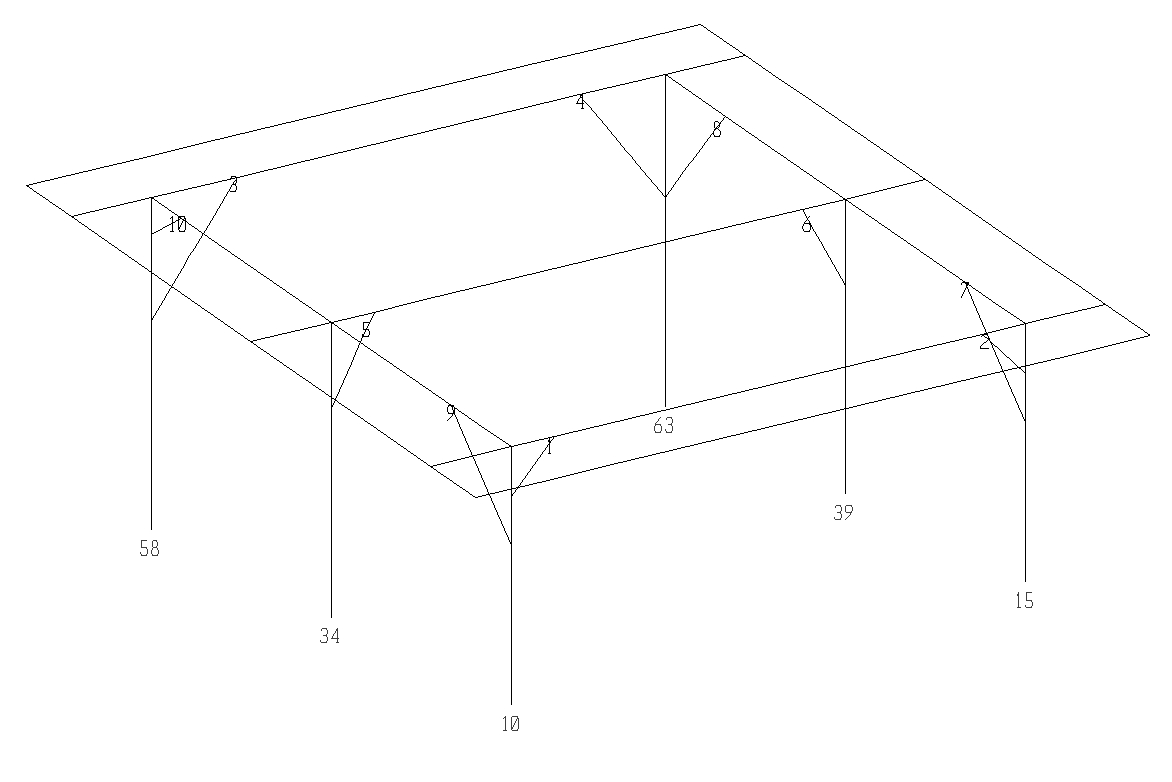
\includegraphics[width=0.700\linewidth]{C:/Users/rodhh/Dropbox/projects/residence_remodel/rivtcalcs0001/docs/d03_models/elements.jpg}\hfill}

\textbf{Column and Brace Numbers} \hfill {[} Fig: 0302.01 {]}

\noindent{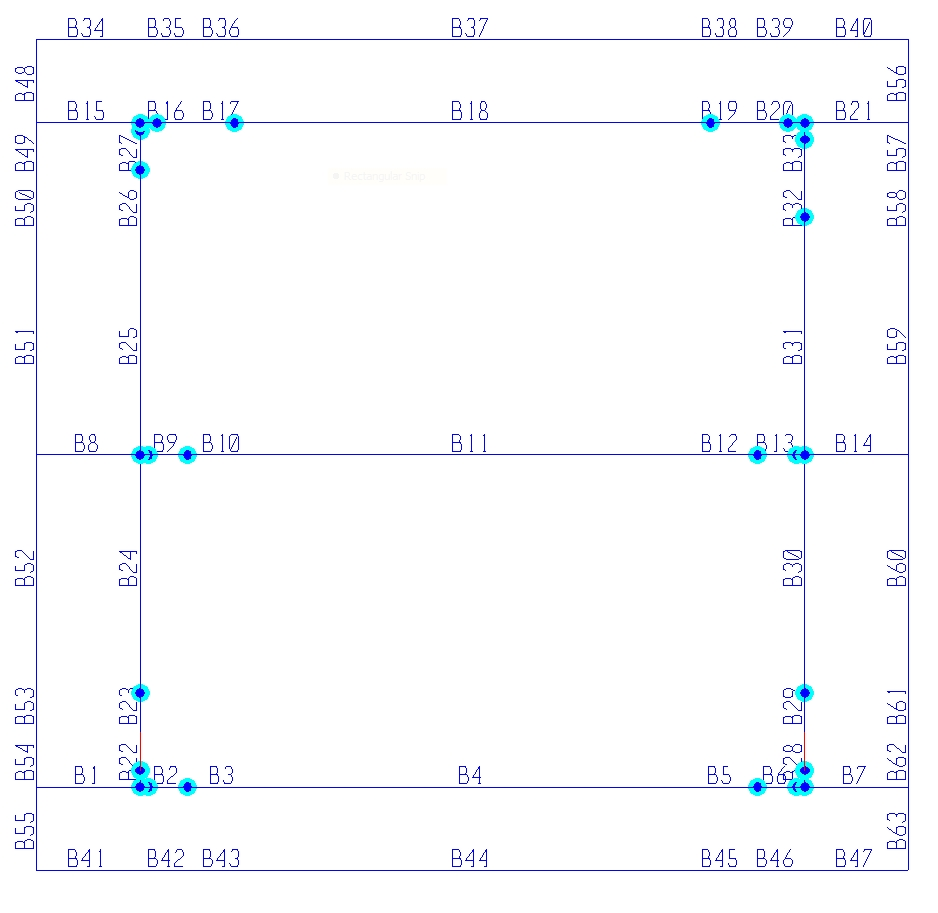
\includegraphics[width=0.500\linewidth]{C:/Users/rodhh/Dropbox/projects/residence_remodel/rivtcalcs0001/docs/d03_models/beams2.jpg}\hfill}

\textbf{Beam Numbers} \hfill {[} Fig: 0302.02 {]}

\noindent{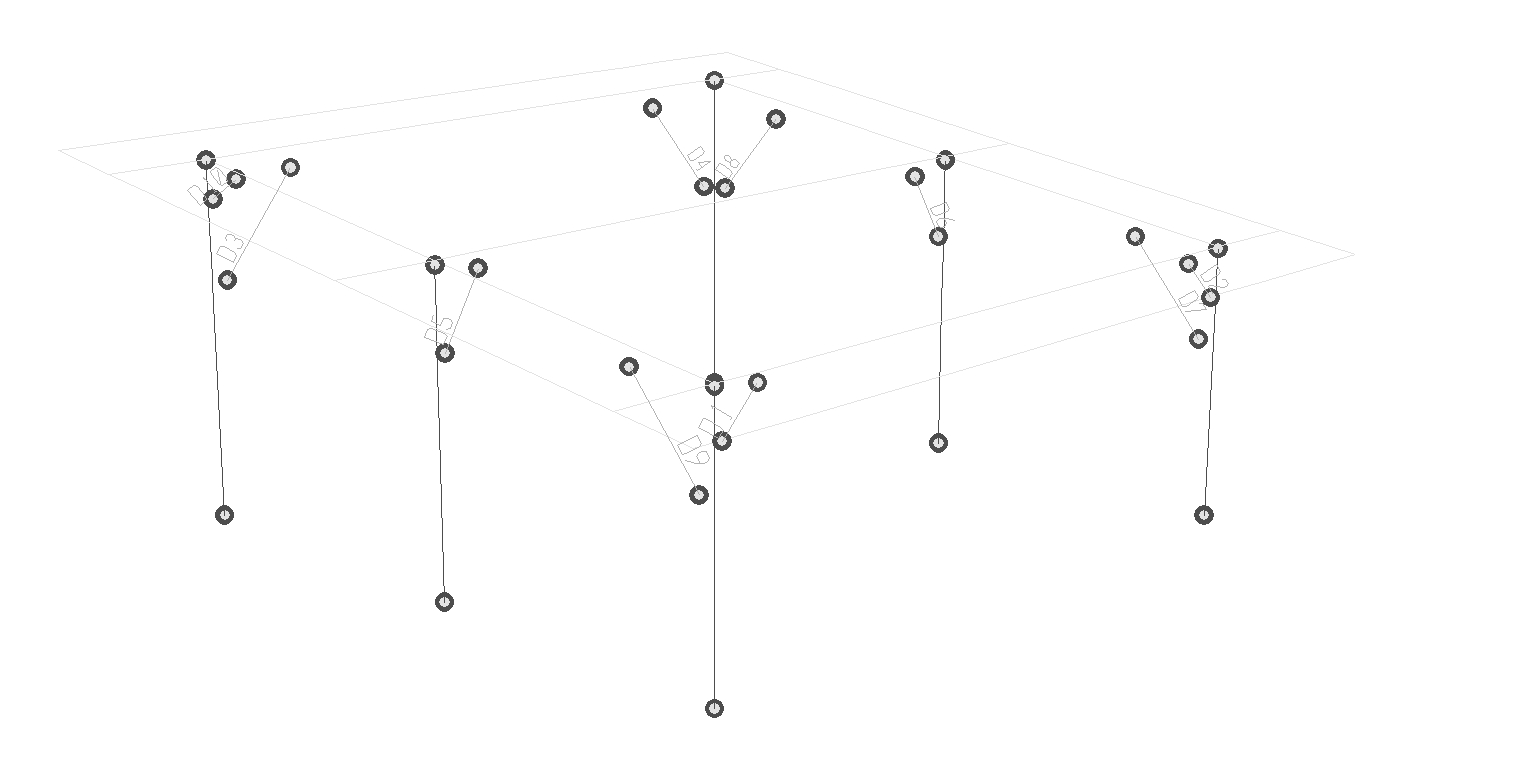
\includegraphics[width=0.900\linewidth]{C:/Users/rodhh/Dropbox/projects/residence_remodel/rivtcalcs0001/docs/d03_models/pins.jpg}\hfill}

\textbf{Element Pin Connections} \hfill {[} Fig: 0302.03 {]}

\noindent{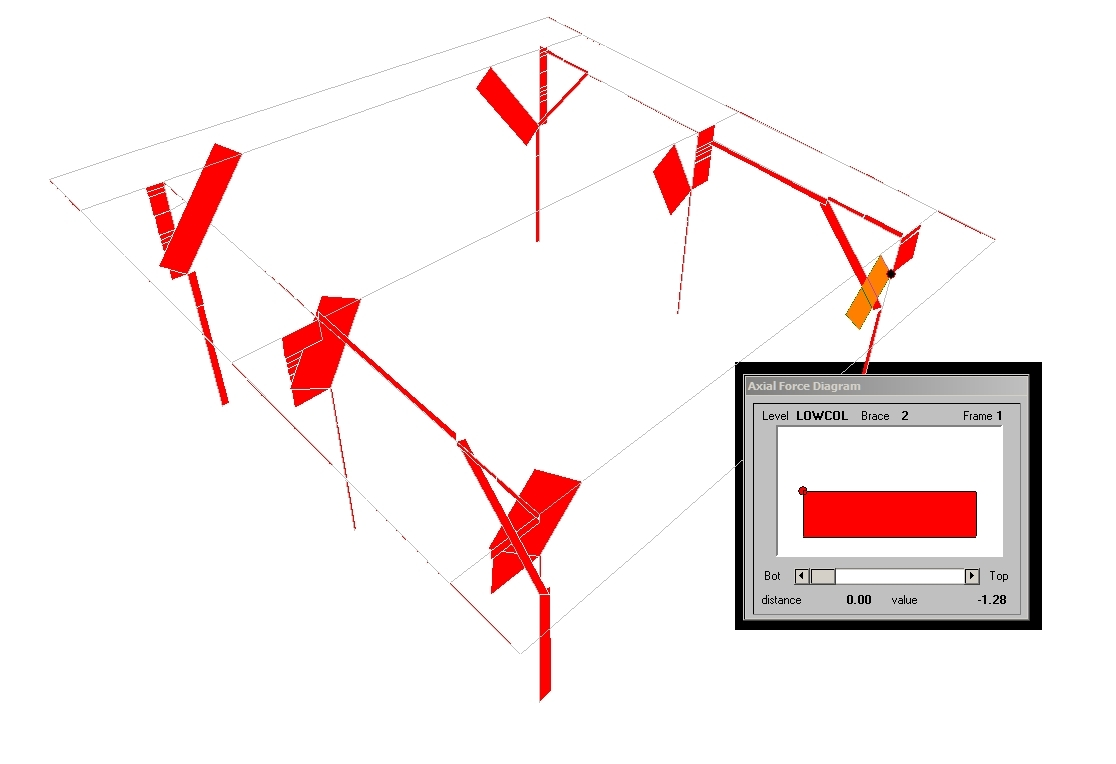
\includegraphics[width=0.900\linewidth]{C:/Users/rodhh/Dropbox/projects/residence_remodel/rivtcalcs0001/docs/d03_models/forceA.jpg}\hfill}

\textbf{Axial Forces - Transverse Seismic} \hfill {[} Fig: 0302.04 {]}

\noindent{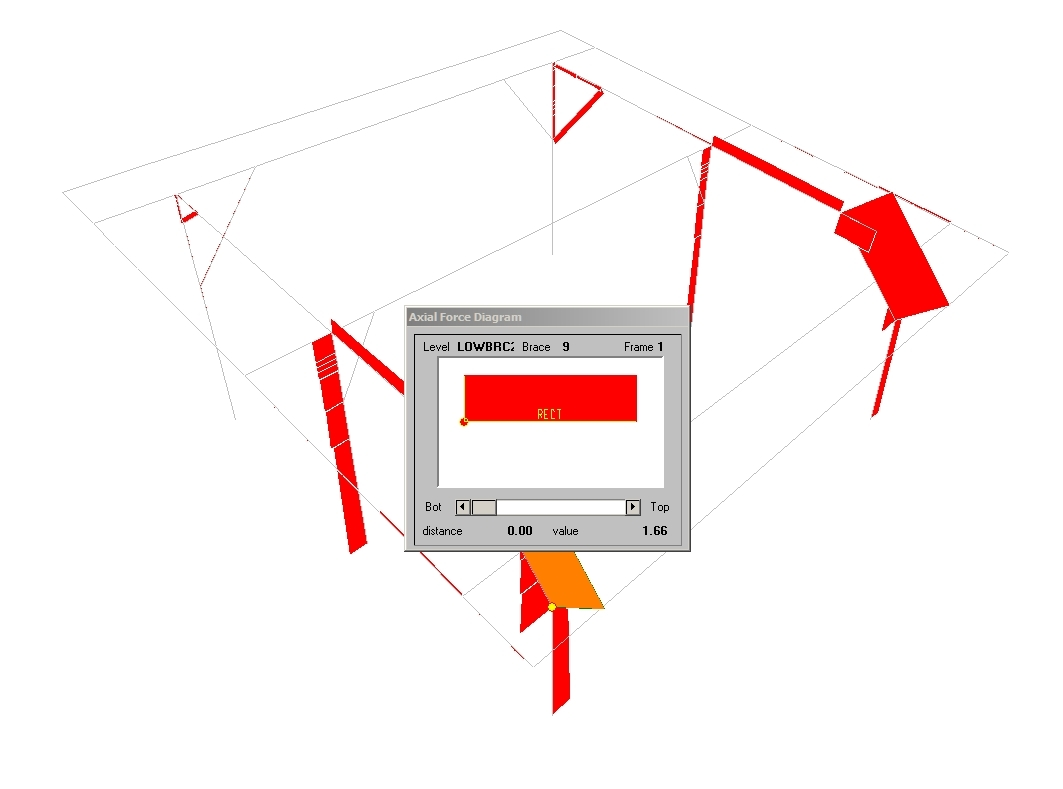
\includegraphics[width=0.900\linewidth]{C:/Users/rodhh/Dropbox/projects/residence_remodel/rivtcalcs0001/docs/d03_models/forceB.jpg}\hfill}

\textbf{Axial Forces - Longitudinal Seismic} \hfill {[} Fig: 0302.05 {]}

\noindent{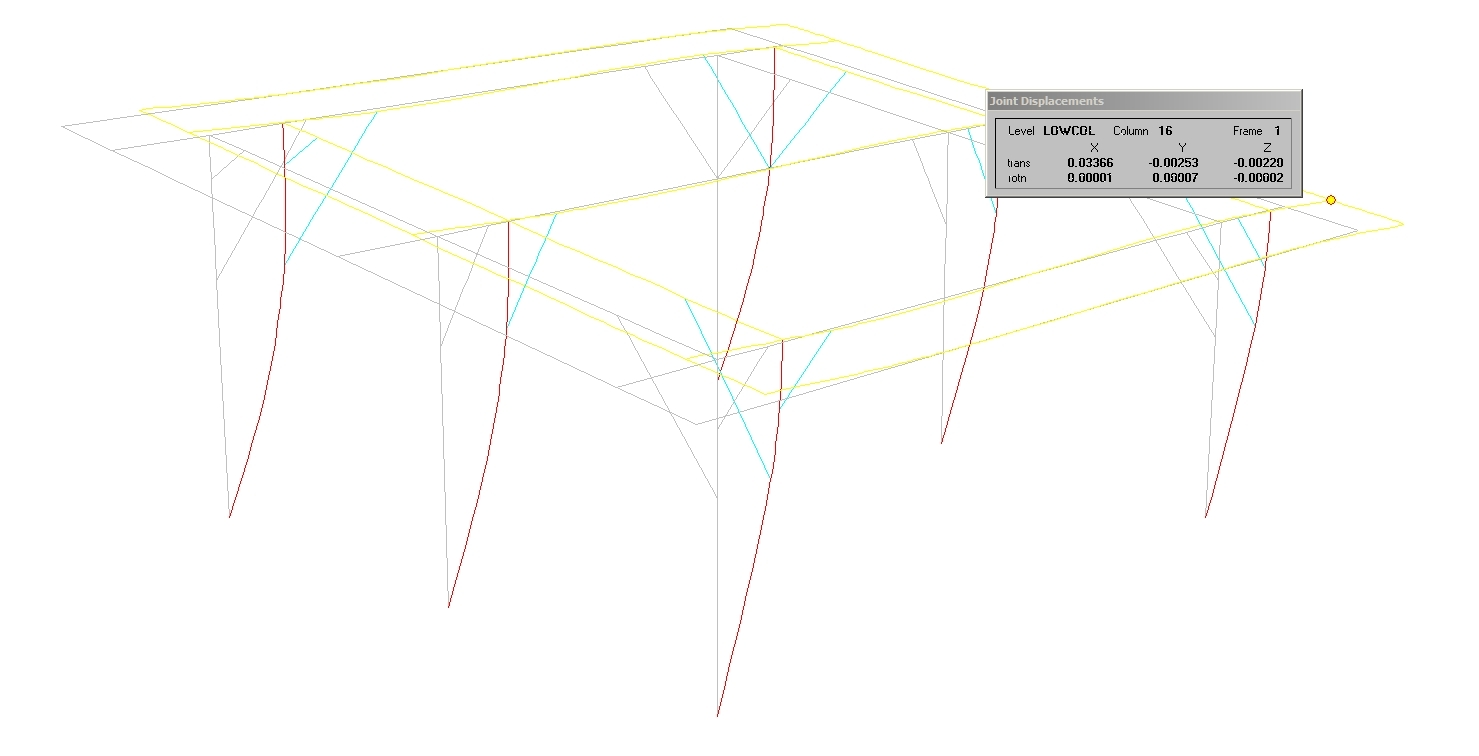
\includegraphics[width=0.900\linewidth]{C:/Users/rodhh/Dropbox/projects/residence_remodel/rivtcalcs0001/docs/d03_models/deltA.jpg}\hfill}

\textbf{Deformations - Transverse Seismic (visually amplified)} \hfill {[} Fig: 0302.06 {]}

\noindent{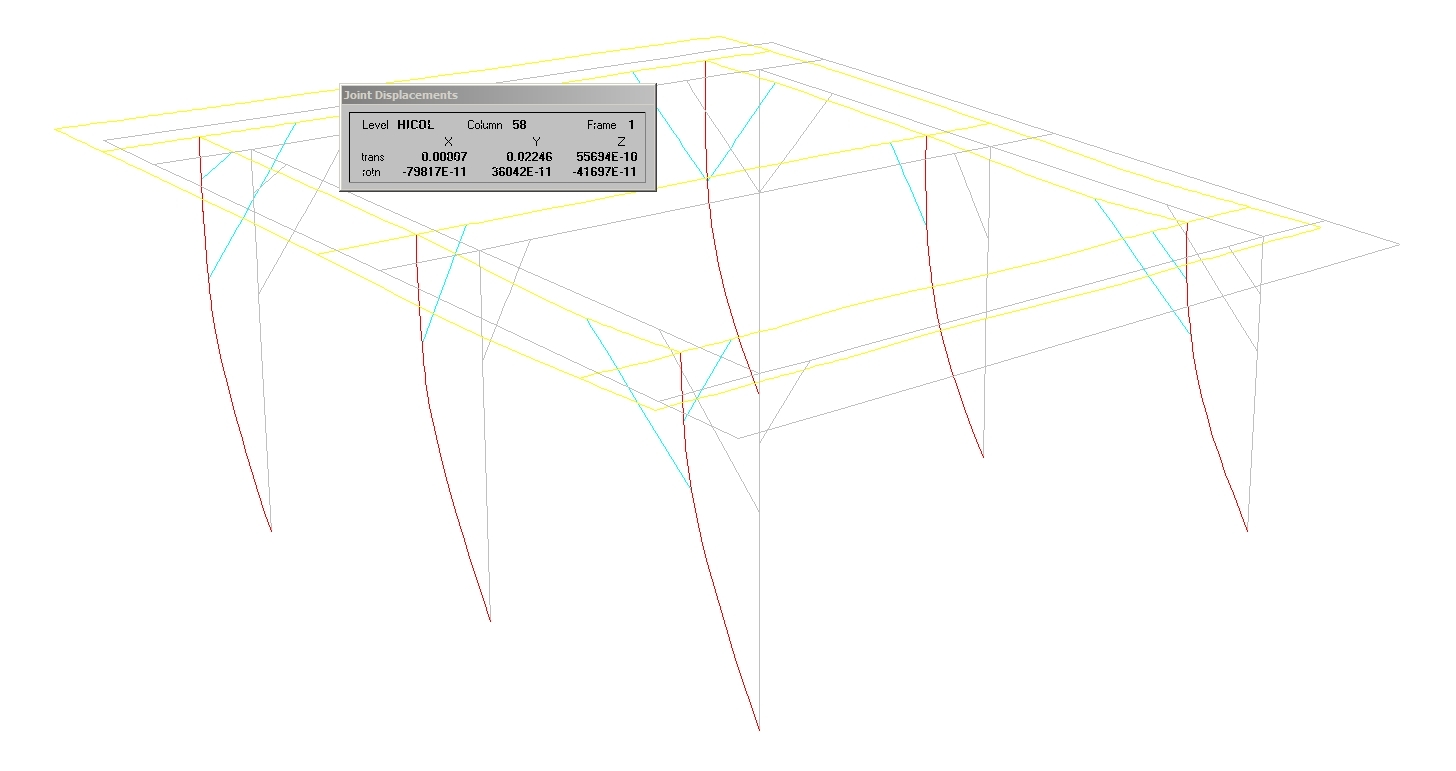
\includegraphics[width=0.900\linewidth]{C:/Users/rodhh/Dropbox/projects/residence_remodel/rivtcalcs0001/docs/d03_models/deltB.jpg}\hfill}

\textbf{Deformations - Longitudinal Seismic (visually amplified)} \hfill {[} Fig: 0302.07 {]}

\begin{quote}
\begin{alltt}
                                E T A B S
            Extended Three Dimensional Analysis of Building Systems
                           NONLINEAR Version 6.22
                           Copyright (C) 1983-1998
                        COMPUTERS AND STRUCTURES, INC.
                              All rights reserved

CARPORT
SEISMIC ANALYSIS
J O B   C O N T R O L   I N F O R M A T I O N
NUMBER OF STORIES----------------------------  11
NUMBER OF FLOOR DIAPHRAGMS ON EACH LEVEL-----   1
NUMBER OF DIFFERENT FRAMES-------------------   1
NUMBER OF TOTAL FRAMES-----------------------   1
NUMBER OF MASS TYPES-------------------------   0
NUMBER OF LOAD CASES-------------------------   0
NUMBER OF STRUCTURAL PERIODS-----------------   3
NUMBER OF MATERIAL PROPERTIES----------------   1
NUMBER OF PROPERTIES FOR COLUMNS-------------   1
NUMBER OF PROPERTIES FOR BEAMS---------------   2
NUMBER OF PROPERTIES FOR FLOORS--------------   1
NUMBER OF PROPERTIES FOR BRACES--------------   1
NUMBER OF PROPERTIES FOR PANELS--------------   0
NUMBER OF PROPERTIES FOR SUPPORTS/LINKS------   0
CODE FOR STATIC LATERAL ANALYSIS-------------  11
CODE FOR DYNAMIC LATERAL ANALYSIS------------   1
CODE FOR STRUCTURE TYPE----------------------   0
CODE FOR P-DELTA ANALYSIS -------------------   0
CODE FOR FRAME JOINT STIFFNESS MODIFICATION--   2
CODE FOR FRAME SELF WEIGHT LOAD CONDITION----   0
CODE FOR TYPE OF UNITS-----------------------   1
GRAVITATIONAL ACCELERATION-----------------   0.3864E+03
EIGEN CONVERGENCE TOLERANCE----------------   0.1000E-03
EIGEN CUTOFF TIME PERIOD-------------------   0.0000E+00
P-DELTA FACTOR-----------------------------   0.1000E+01
CARPORT
SEISMIC ANALYSIS
STRUCTURAL STORY DATA . . .
STORY         STORY  NUMBER OF
LEVEL        HEIGHT DIAPHRAGMS
HITRIM         3.00          0
HICOL          2.00          0
HIBRAC1        2.00          0
HIBRAC2        8.00          0
MIDCOL         8.00          0
LOWBRC2        2.00          0
LOWBRC1        2.00          0
LOWCOL         3.00          0
LOWTRIM       13.00          0
LOWBC1        16.00          0
LOWBC2        52.00          0
CARPORT
SEISMIC ANALYSIS
MATERIAL PROPERTIES
ID TYPE     ELASTIC    POISSONS        UNIT        UNIT    COEFF OF
            MODULUS       RATIO      WEIGHT        MASS   EXPANSION
   1    O  0.1000E+05      0.3000  0.2300E-04  0.6000E-07  0.0000E+00
MATERIAL PROPERTIES FOR DESIGN
ID TYPE         FY         FC        FYS        FCS      FBMAJ      FBMIN

SECTION PROPERTIES FOR COLUMNS
      SECTION            MAT     MAJOR     MINOR    FLANGE       WEB
   ID  TYPE                ID       DIM       DIM     THICK     THICK
   1  RECT                 1     5.500     5.500     0.000     0.000
SECTION PROPERTY REDUCTION FACTORS FOR  COLUMNS
            TORSION       MAJOR       MINOR
   ID             J           I           I
   1         1.000       1.000       1.000
ANALYSIS SECTION PROPERTIES FOR   COLUMNS
            AXIAL       MAJOR       MINOR     TORSION       MAJOR       MINOR
   ID             A          AV          AV           J           I           I
   1        30.250      25.208      25.208  0.1289E+03  0.7626E+02  0.7626E+02

SECTION PROPERTIES FOR BEAMS
      SECTION            MAT     DEPTH     DEPTH      BEAM    FLANGE       WEB
   ID  TYPE                ID     BELOW     ABOVE     WIDTH     THICK     THICK
   1  RECT                 1    11.250     0.000     3.500     0.000     0.000
   2  RECT                 1     5.500     0.000     1.500     0.000     0.000
SECTION PROPERTY REDUCTION FACTORS FOR  BEAMS
            TORSION       MAJOR       MINOR
   ID             J           I           I
   1         1.000       1.000       1.000
   2         1.000       1.000       1.000
ANALYSIS SECTION PROPERTIES FOR   BEAMS
            AXIAL       MAJOR       MINOR     TORSION       MAJOR       MINOR
   ID             A          AV          AV           J           I           I
   1        39.375      32.813      32.813  0.1293E+03  0.4153E+03  0.4020E+02
   2         8.250       6.875       6.875  0.5125E+01  0.2080E+02  0.1547E+01
CARPORT
SEISMIC ANALYSIS
SECTION PROPERTIES FOR   FLOORS
      ELEMENT   MAT    FLOOR    FLOOR    FLOOR
   ID TYPE       ID      T11      T22      T12
   1 MEMB        1    1.500    1.500    0.100
CARPORT
SEISMIC ANALYSIS
SECTION PROPERTIES FOR BRACES
      SECTION            MAT     MAJOR     MINOR    FLANGE       WEB
   ID  TYPE                ID       DIM       DIM     THICK     THICK
   1  RECT                 1     3.500     3.500     0.000     0.000
SECTION PROPERTY REDUCTION FACTORS FOR  BRACES
            TORSION       MAJOR       MINOR
   ID             J           I           I
   1         1.000       1.000       1.000
ANALYSIS SECTION PROPERTIES FOR   BRACES
            AXIAL       MAJOR       MINOR     TORSION       MAJOR       MINOR
   ID             A          AV          AV           J           I           I
   1        12.250      10.208      10.208  0.2113E+02  0.1251E+02  0.1251E+02
CARPORT
SEISMIC ANALYSIS
F R A M E   C O N T R O L   I N F O R M A T I O N
CARPORT
FRAME ID NUMBER----------------------------    1
NUMBER OF COLUMN LINES---------------------   72
NUMBER OF BEAM BAYS------------------------   63
NUMBER OF FLOOR BAYS-----------------------   24
NUMBER OF JOINT LOAD PATTERNS--------------    0
NUMBER OF BEAM SPAN LOAD PATTERNS----------    0
NUMBER OF FLOOR SURFACE LOAD PATTERNS------    0
CODE FOR JOINT DATA------------------------    0
MAXIMUM NUMBER OF BRACE ELEMENTS-----------   10
MAXIMUM NUMBER OF PANEL ELEMENTS-----------    0
MAXIMUM NUMBER OF LINK  ELEMENTS-----------    0
MAXIMUM NUMBER OF LOADS PER BEAM SPAN------    4
SEISMIC ANALYSIS
INPUT AND/OR GENERATED BRACING DATA
BRACE  LEVEL      COLUMN   COLUMN     PROP  PIN END   LEVELS           BRACE
   ID  AT TOP     AT BOT   AT TOP       ID  MAJ/MIN  DROPPED          LENGTH
   1  LOWCOL         10       11        1      3/3        2           22.63
   2  LOWCOL         15       14        1      3/3        2           22.63
   3  HICOL          58       60        1      3/3        8           51.22
   4  HICOL          63       61        1      3/3        8           51.22
   5  MIDCOL         34       35        1      3/3        5           32.25
   6  MIDCOL         39       38        1      3/3        5           32.25
   7  LOWBRC2        15       31        1      3/3        5           48.17
   8  HIBRAC2        63       47        1      3/3        6           48.17
   9  LOWBRC2        10       26        1      3/3        5           48.17
   10  HIBRAC1        58       50        1      3/3        2           18.87
LEVEL    /------------------ELEMENT TYPE-----------------/
ID          COLUMN      BEAM     BRACE     PANEL     FLOOR
HITRIM       0.000     0.052     0.000     0.000     0.105
HICOL        0.001     0.241     0.014     0.000     0.175
HIBRAC1      0.003     0.035     0.003     0.000     0.140
HIBRAC2      0.007     0.088     0.007     0.000     0.350
MIDCOL       0.017     0.360     0.012     0.000     0.561
LOWBRC2      0.014     0.088     0.014     0.000     0.350
LOWBRC1      0.006     0.035     0.000     0.000     0.140
LOWCOL       0.009     0.241     0.006     0.000     0.175
LOWTRIM      0.033     0.052     0.000     0.000     0.105
LOWBC1       0.061     0.000     0.037     0.000     0.000
LOWBC2       0.142     0.000     0.014     0.000     0.000
BASELINE     0.109     0.000     0.000     0.000     0.000
TOTALS   0.401E+00 0.119E+01 0.106E+00 0.000E+00 0.210E+01
CARPORT
SEISMIC ANALYSIS
DIAPHRAGM MASS DATA
RESULTANTS OF STORY & TRIBUTARY ELEMENT MASSES
STORY     DIAPHRAGM   DIAPHRAGM   DIAPHRAGM   DIAPHRAGM   DIAPHRAGM
LEVEL        NUMBER        MASS         MMI         X-M         Y-M
HITRIM
                  1       0.000  0.3774E+01      126.00      240.00
HICOL
                  1       0.001  0.9170E+01      126.00      216.00
HIBRAC1
                  1       0.000  0.4748E+01      124.59      200.25
HIBRAC2
                  1       0.001  0.1189E+02      127.44      184.49
MIDCOL
                  1       0.002  0.2315E+02      125.73      121.40
LOWBRC2
                  1       0.001  0.1273E+02      126.00       59.34
LOWBRC1
                  1       0.000  0.5014E+01      126.00       43.93
LOWCOL
                  1       0.001  0.9719E+01      126.00       26.32
LOWTRIM
                  1       0.000  0.6148E+01      126.00       20.99
LOWBC1
                  1       0.000  0.3905E+01      132.70      134.66
LOWBC2
                  1       0.000  0.6311E+01      126.00      111.62
CARPORT
SEISMIC ANALYSIS
STATIC SEISMIC LOAD CALCULATION DATA . . .
UNIFORM BUILDING CODE 1994
UBC ZONE FACTOR (Z)-------------------------      0.40
UBC IMPORTANCE FACTOR (I)-------------------      1.00
UBC SITE COEFFICIENT (S) -------------------      1.20
LOAD CONDITION A (X-DIRECTION) . . .
PERIOD OF PREDOMINANT X STRUCTURAL MODE-----     0.500
UBC (METHOD A) PERIOD FOR X DIRECTION-------     0.500
UBC STRUCTURAL SYSTEM COEFFICIENT (RW)------     4.000
TOP    LEVEL OF TRIANGULAR DISTRIBUTION-----  HITRIM
BOTTOM LEVEL OF TRIANGULAR DISTRIBUTION-----  BASELINE
LOAD CONDITION B (Y-DIRECTION) . . .
PERIOD OF PREDOMINANT Y STRUCTURAL MODE-----     0.500
UBC (METHOD A) PERIOD FOR Y DIRECTION-------     0.500
UBC STRUCTURAL SYSTEM COEFFICIENT (RW)------     4.000
TOP    LEVEL OF TRIANGULAR DISTRIBUTION-----  HITRIM
BOTTOM LEVEL OF TRIANGULAR DISTRIBUTION-----  BASELINE
ADDITIONAL STORY ECCENTRICITIES . . .
LEVEL           EYA        EXB
HITRIM         0.00       0.00
HICOL          0.00       0.00
HIBRAC1        0.00       0.00
HIBRAC2        0.00       0.00
MIDCOL         0.00       0.00
LOWBRC2        0.00       0.00
LOWBRC1        0.00       0.00
LOWCOL         0.00       0.00
LOWTRIM        0.00       0.00
LOWBC1         0.00       0.00
LOWBC2         0.00       0.00
CARPORT
SEISMIC ANALYSIS
UBC '94 SEISMIC LOADS FOR DIRECTION   X
V = ZICW/RW,   C = 1.25S/T**(2/3)
T =    0.5000
Z =    0.4000
S =    1.2000
I =    1.0000
C =    2.3811
RW=    4.0000
W =       3.7
V =    0.2381W
   =      0.89
FT=      0.00
CARPORT
SEISMIC ANALYSIS
UBC '94 SEISMIC LOADS FOR DIRECTION   Y
V = ZICW/RW,   C = 1.25S/T**(2/3)
T =    0.5000
Z =    0.4000
S =    1.2000
I =    1.0000
C =    2.3811
RW=    4.0000
W =       3.7
V =    0.2381W
   =      0.89
FT=      0.00
CARPORT
SEISMIC ANALYSIS
STRUCTURAL LATERAL LOAD CONDITIONS
AS ADJUSTED BY CODE SEISMIC REQUIREMENTS
STRUCTURAL LATERAL LOAD CONDITION A (X-DIRECTION) FOR DIAPHRAGM     1
LEVEL             FX          FY           X           Y
HITRIM          0.05        0.00      126.00      240.00
HICOL           0.12        0.00      126.00      216.00
HIBRAC1         0.05        0.00      124.59      200.25
HIBRAC2         0.12        0.00      127.44      184.49
MIDCOL          0.23        0.00      125.73      121.40
LOWBRC2         0.11        0.00      126.00       59.34
LOWBRC1         0.04        0.00      126.00       43.93
LOWCOL          0.09        0.00      126.00       26.32
LOWTRIM         0.04        0.00      126.00       20.99
LOWBC1          0.02        0.00      132.70      134.66
LOWBC2          0.02        0.00      126.00      111.62
CARPORT
STRUCTURAL LATERAL LOAD CONDITION B (Y-DIRECTION) FOR DIAPHRAGM     1
LEVEL             FX          FY           X           Y
HITRIM          0.00        0.05      126.00      240.00
HICOL           0.00        0.12      126.00      216.00
HIBRAC1         0.00        0.05      124.59      200.25
HIBRAC2         0.00        0.12      127.44      184.49
MIDCOL          0.00        0.23      125.73      121.40
LOWBRC2         0.00        0.11      126.00       59.34
LOWBRC1         0.00        0.04      126.00       43.93
LOWCOL          0.00        0.09      126.00       26.32
LOWTRIM         0.00        0.04      126.00       20.99
LOWBC1          0.00        0.02      132.70      134.66
LOWBC2          0.00        0.02      126.00      111.62
CARPORT
STRUCTURAL LATERAL LOAD CONDITION C (ROTATION) FOR DIAPHRAGM     1
LEVEL             MZ
HITRIM          0.00
HICOL           0.00
HIBRAC1         0.00
HIBRAC2         0.00
MIDCOL          0.00
LOWBRC2         0.00
LOWBRC1         0.00
LOWCOL          0.00
LOWTRIM         0.00
LOWBC1          0.00
LOWBC2          0.00
\end{alltt}
\end{quote}

\begin{quote}
\begin{alltt}
SEISMIC ANALYSIS
COORDINATES OF CENTERS OF CUMULATIVE MASS & CENTERS OF RIGIDITY
STORY  DIAPHRAGM /----------CENTER OF MASS----------//--CENTER OF RIGIDITY--/
LEVEL     NUMBER        MASS  ORDINATE-X  ORDINATE-Y  ORDINATE-X  ORDINATE-Y
HITRIM
                1       0.000     126.000     240.000     126.237     116.614
HICOL
                1       0.002     126.000     222.418     126.451     114.938
HIBRAC1
                1       0.002     125.669     217.208     126.590     114.735
HIBRAC2
                1       0.003     126.324     205.099     126.682     114.562
MIDCOL
                1       0.006     126.065     168.525     126.433     114.186
LOWBRC2
                1       0.007     126.053     149.224     126.382     114.455
LOWBRC1
                1       0.007     126.050     142.460     126.366     114.476
LOWCOL
                1       0.008     126.043     127.052     126.345     114.502
LOWTRIM
                1       0.009     126.041     121.166     126.295     114.701
LOWBC1
                1       0.009     126.224     121.537     126.104     116.163
LOWBC2
                1       0.010     126.215     121.120     126.055     117.272


STATIC LOAD CONDITION LATERAL STORY SHEARS FOR ALL DIAPHRAGMS
VALUES ARE AT THE GLOBAL ORIGIN IN THE GLOBAL COORDINATES
                /---------------------LOAD  CONDITIONS---------------------/
LEVEL     DIRN           I        II       III         A         B         C
HITRIM       X        0.00      0.00      0.00      0.05      0.00      0.00
HITRIM       Y        0.00      0.00      0.00      0.00      0.05      0.00
HICOL        X        0.00      0.00      0.00      0.16      0.00      0.00
HICOL        Y        0.00      0.00      0.00      0.00      0.16      0.00
HIBRAC1      X        0.00      0.00      0.00      0.21      0.00      0.00
HIBRAC1      Y        0.00      0.00      0.00      0.00      0.21      0.00
HIBRAC2      X        0.00      0.00      0.00      0.34      0.00      0.00
HIBRAC2      Y        0.00      0.00      0.00      0.00      0.34      0.00
MIDCOL       X        0.00      0.00      0.00      0.57      0.00      0.00
MIDCOL       Y        0.00      0.00      0.00      0.00      0.57      0.00
LOWBRC2      X        0.00      0.00      0.00      0.68      0.00      0.00
LOWBRC2      Y        0.00      0.00      0.00      0.00      0.68      0.00
LOWBRC1      X        0.00      0.00      0.00      0.72      0.00      0.00
LOWBRC1      Y        0.00      0.00      0.00      0.00      0.72      0.00
LOWCOL       X        0.00      0.00      0.00      0.81      0.00      0.00
LOWCOL       Y        0.00      0.00      0.00      0.00      0.81      0.00
LOWTRIM      X        0.00      0.00      0.00      0.85      0.00      0.00
LOWTRIM      Y        0.00      0.00      0.00      0.00      0.85      0.00
LOWBC1       X        0.00      0.00      0.00      0.87      0.00      0.00
LOWBC1       Y        0.00      0.00      0.00      0.00      0.87      0.00
LOWBC2       X        0.00      0.00      0.00      0.89      0.00      0.00
LOWBC2       Y        0.00      0.00      0.00      0.00      0.89      0.00
CARPORT

STATIC LOAD CONDITION LATERAL FRAME DRIFT RATIOS  FOR DIAPHRAGM    1
VALUES ARE AT THE FRAME ORIGIN IN THE FRAME LOCAL COORDINATES
                /---------------------LOAD  CONDITIONS---------------------/
LEVEL     DIRN           I        II       III         A         B         C
HITRIM       X     0.00000   0.00000   0.00000   0.00002   0.00001   0.00000
HITRIM       Y     0.00000   0.00000   0.00000   0.00000   0.00001   0.00000
HITRIM    ROTZ     0.00000   0.00000   0.00000   0.00000   0.00000   0.00000
HICOL        X     0.00000   0.00000   0.00000   0.00000   0.00001   0.00000
HICOL        Y     0.00000   0.00000   0.00000   0.00000   0.00000   0.00000
HICOL     ROTZ     0.00000   0.00000   0.00000   0.00000   0.00000   0.00000
HIBRAC1      X     0.00000   0.00000   0.00000   0.00000   0.00001   0.00000
HIBRAC1      Y     0.00000   0.00000   0.00000   0.00000   0.00000   0.00000
HIBRAC1   ROTZ     0.00000   0.00000   0.00000   0.00000   0.00000   0.00000
HIBRAC2      X     0.00000   0.00000   0.00000   0.00001  -0.00001   0.00000
HIBRAC2      Y     0.00000   0.00000   0.00000   0.00000   0.00000   0.00000
HIBRAC2   ROTZ     0.00000   0.00000   0.00000   0.00000   0.00000   0.00000
MIDCOL       X     0.00000   0.00000   0.00000   0.00003   0.00000   0.00000
MIDCOL       Y     0.00000   0.00000   0.00000   0.00000  -0.00002   0.00000
MIDCOL    ROTZ     0.00000   0.00000   0.00000   0.00000   0.00000   0.00000
LOWBRC2      X     0.00000   0.00000   0.00000   0.00003   0.00000   0.00000
LOWBRC2      Y     0.00000   0.00000   0.00000   0.00001   0.00003   0.00000
LOWBRC2   ROTZ     0.00000   0.00000   0.00000   0.00000   0.00000   0.00000
LOWBRC1      X     0.00000   0.00000   0.00000   0.00004   0.00000   0.00000
LOWBRC1      Y     0.00000   0.00000   0.00000   0.00001   0.00005   0.00000
LOWBRC1   ROTZ     0.00000   0.00000   0.00000   0.00000   0.00000   0.00000
LOWCOL       X     0.00000   0.00000   0.00000   0.00005   0.00000   0.00000
LOWCOL       Y     0.00000   0.00000   0.00000   0.00001   0.00003   0.00000
LOWCOL    ROTZ     0.00000   0.00000   0.00000   0.00000   0.00000   0.00000
LOWTRIM      X     0.00000   0.00000   0.00000   0.00011   0.00000   0.00000
LOWTRIM      Y     0.00000   0.00000   0.00000   0.00002   0.00005   0.00000
LOWTRIM   ROTZ     0.00000   0.00000   0.00000   0.00000   0.00000   0.00000
LOWBC1       X     0.00000   0.00000   0.00000   0.00027   0.00000   0.00000
LOWBC1       Y     0.00000   0.00000   0.00000   0.00002   0.00013   0.00000
LOWBC1    ROTZ     0.00000   0.00000   0.00000   0.00000   0.00000   0.00000
LOWBC2       X     0.00000   0.00000   0.00000   0.00052   0.00000   0.00000
LOWBC2       Y     0.00000   0.00000   0.00000   0.00004   0.00038   0.00000
LOWBC2    ROTZ     0.00000   0.00000   0.00000   0.00000   0.00000   0.00000
\end{alltt}
\end{quote}

\begin{quote}
\begin{alltt}
STRUCTURAL TIME PERIODS AND FREQUENCIES
MODE                   PERIOD           FREQUENCY       CIRCULAR/FREQ
NUMBER                   (TIME)  (CYCLES/UNIT TIME) (RADIANS/UNIT TIME)
     1                  0.12353             8.09552            50.86566
     2                  0.09821            10.18244            63.97819
     3                  0.09772            10.23350            64.29899
MODAL PARTICIPATION FACTORS
MODE                  X-TRANS             Y-TRANS              Z-ROTN
NUMBER                DIRECTION           DIRECTION           DIRECTION
     1                  0.09758             0.00029            -0.78367
     2                 -0.00983             0.01423            -7.91733
     3                  0.00115             0.09709             1.16317
MODAL DIRECTION FACTORS
MODE                  X-TRANS             Y-TRANS              Z-ROTN
NUMBER                DIRECTION           DIRECTION           DIRECTION
     1                 99.36060             0.00096             0.63844
     2                 32.87273             2.11559            65.01169
     3                  0.70362            97.89345             1.40293
EFFECTIVE MASS FACTORS
NUMBER        %-MASS  <%-SUM>     %-MASS  <%-SUM>     %-MASS  <%-SUM>
     1         98.83  < 98.8>       0.00  <  0.0>       0.64  <  0.6>
     2          1.00  < 99.8>       2.10  <  2.1>      64.93  < 65.6>
     3          0.01  < 99.8>      97.83  < 99.9>       1.40  < 67.0>
\end{alltt}
\end{quote}

\begin{quote}
\begin{alltt}
SEISMIC ANALYSIS
COORDINATES OF CENTERS OF CUMULATIVE MASS & CENTERS OF RIGIDITY
STORY  DIAPHRAGM /----------CENTER OF MASS----------//--CENTER OF RIGIDITY--/
LEVEL     NUMBER        MASS  ORDINATE-X  ORDINATE-Y  ORDINATE-X  ORDINATE-Y
HITRIM
                1       0.000     126.000     240.000     126.237     116.614
HICOL
                1       0.002     126.000     222.418     126.451     114.938
HIBRAC1
                1       0.002     125.669     217.208     126.590     114.735
HIBRAC2
                1       0.003     126.324     205.099     126.682     114.562
MIDCOL
                1       0.006     126.065     168.525     126.433     114.186
LOWBRC2
                1       0.007     126.053     149.224     126.382     114.455
LOWBRC1
                1       0.007     126.050     142.460     126.366     114.476
LOWCOL
                1       0.008     126.043     127.052     126.345     114.502
LOWTRIM
                1       0.009     126.041     121.166     126.295     114.701
LOWBC1
                1       0.009     126.224     121.537     126.104     116.163
LOWBC2
                1       0.010     126.215     121.120     126.055     117.272


STATIC LOAD CONDITION LATERAL STORY SHEARS FOR ALL DIAPHRAGMS
VALUES ARE AT THE GLOBAL ORIGIN IN THE GLOBAL COORDINATES
                /---------------------LOAD  CONDITIONS---------------------/
LEVEL     DIRN           I        II       III         A         B         C
HITRIM       X        0.00      0.00      0.00      0.05      0.00      0.00
HITRIM       Y        0.00      0.00      0.00      0.00      0.05      0.00
HICOL        X        0.00      0.00      0.00      0.16      0.00      0.00
HICOL        Y        0.00      0.00      0.00      0.00      0.16      0.00
HIBRAC1      X        0.00      0.00      0.00      0.21      0.00      0.00
HIBRAC1      Y        0.00      0.00      0.00      0.00      0.21      0.00
HIBRAC2      X        0.00      0.00      0.00      0.34      0.00      0.00
HIBRAC2      Y        0.00      0.00      0.00      0.00      0.34      0.00
MIDCOL       X        0.00      0.00      0.00      0.57      0.00      0.00
MIDCOL       Y        0.00      0.00      0.00      0.00      0.57      0.00
LOWBRC2      X        0.00      0.00      0.00      0.68      0.00      0.00
LOWBRC2      Y        0.00      0.00      0.00      0.00      0.68      0.00
LOWBRC1      X        0.00      0.00      0.00      0.72      0.00      0.00
LOWBRC1      Y        0.00      0.00      0.00      0.00      0.72      0.00
LOWCOL       X        0.00      0.00      0.00      0.81      0.00      0.00
LOWCOL       Y        0.00      0.00      0.00      0.00      0.81      0.00
LOWTRIM      X        0.00      0.00      0.00      0.85      0.00      0.00
LOWTRIM      Y        0.00      0.00      0.00      0.00      0.85      0.00
LOWBC1       X        0.00      0.00      0.00      0.87      0.00      0.00
LOWBC1       Y        0.00      0.00      0.00      0.00      0.87      0.00
LOWBC2       X        0.00      0.00      0.00      0.89      0.00      0.00
LOWBC2       Y        0.00      0.00      0.00      0.00      0.89      0.00
CARPORT

STATIC LOAD CONDITION LATERAL FRAME DRIFT RATIOS  FOR DIAPHRAGM    1
VALUES ARE AT THE FRAME ORIGIN IN THE FRAME LOCAL COORDINATES
                /---------------------LOAD  CONDITIONS---------------------/
LEVEL     DIRN           I        II       III         A         B         C
HITRIM       X     0.00000   0.00000   0.00000   0.00002   0.00001   0.00000
HITRIM       Y     0.00000   0.00000   0.00000   0.00000   0.00001   0.00000
HITRIM    ROTZ     0.00000   0.00000   0.00000   0.00000   0.00000   0.00000
HICOL        X     0.00000   0.00000   0.00000   0.00000   0.00001   0.00000
HICOL        Y     0.00000   0.00000   0.00000   0.00000   0.00000   0.00000
HICOL     ROTZ     0.00000   0.00000   0.00000   0.00000   0.00000   0.00000
HIBRAC1      X     0.00000   0.00000   0.00000   0.00000   0.00001   0.00000
HIBRAC1      Y     0.00000   0.00000   0.00000   0.00000   0.00000   0.00000
HIBRAC1   ROTZ     0.00000   0.00000   0.00000   0.00000   0.00000   0.00000
HIBRAC2      X     0.00000   0.00000   0.00000   0.00001  -0.00001   0.00000
HIBRAC2      Y     0.00000   0.00000   0.00000   0.00000   0.00000   0.00000
HIBRAC2   ROTZ     0.00000   0.00000   0.00000   0.00000   0.00000   0.00000
MIDCOL       X     0.00000   0.00000   0.00000   0.00003   0.00000   0.00000
MIDCOL       Y     0.00000   0.00000   0.00000   0.00000  -0.00002   0.00000
MIDCOL    ROTZ     0.00000   0.00000   0.00000   0.00000   0.00000   0.00000
LOWBRC2      X     0.00000   0.00000   0.00000   0.00003   0.00000   0.00000
LOWBRC2      Y     0.00000   0.00000   0.00000   0.00001   0.00003   0.00000
LOWBRC2   ROTZ     0.00000   0.00000   0.00000   0.00000   0.00000   0.00000
LOWBRC1      X     0.00000   0.00000   0.00000   0.00004   0.00000   0.00000
LOWBRC1      Y     0.00000   0.00000   0.00000   0.00001   0.00005   0.00000
LOWBRC1   ROTZ     0.00000   0.00000   0.00000   0.00000   0.00000   0.00000
LOWCOL       X     0.00000   0.00000   0.00000   0.00005   0.00000   0.00000
LOWCOL       Y     0.00000   0.00000   0.00000   0.00001   0.00003   0.00000
LOWCOL    ROTZ     0.00000   0.00000   0.00000   0.00000   0.00000   0.00000
LOWTRIM      X     0.00000   0.00000   0.00000   0.00011   0.00000   0.00000
LOWTRIM      Y     0.00000   0.00000   0.00000   0.00002   0.00005   0.00000
LOWTRIM   ROTZ     0.00000   0.00000   0.00000   0.00000   0.00000   0.00000
LOWBC1       X     0.00000   0.00000   0.00000   0.00027   0.00000   0.00000
LOWBC1       Y     0.00000   0.00000   0.00000   0.00002   0.00013   0.00000
LOWBC1    ROTZ     0.00000   0.00000   0.00000   0.00000   0.00000   0.00000
LOWBC2       X     0.00000   0.00000   0.00000   0.00052   0.00000   0.00000
LOWBC2       Y     0.00000   0.00000   0.00000   0.00004   0.00038   0.00000
LOWBC2    ROTZ     0.00000   0.00000   0.00000   0.00000   0.00000   0.00000
\end{alltt}
\end{quote}

\vspace{.2in}   \textbf{Seismic D-C Ratios for Braces}   \hfill\textbf{SECTION 02}
\newline   \vspace{.05in}   {\color{black}\hrulefill}

Connection capacities evaluated using Woodworks 11.2.  The software does not
allow a single bolt row so a two bolt configuration is analyzed and
capacities are reduced by a factor of 2.

\noindent{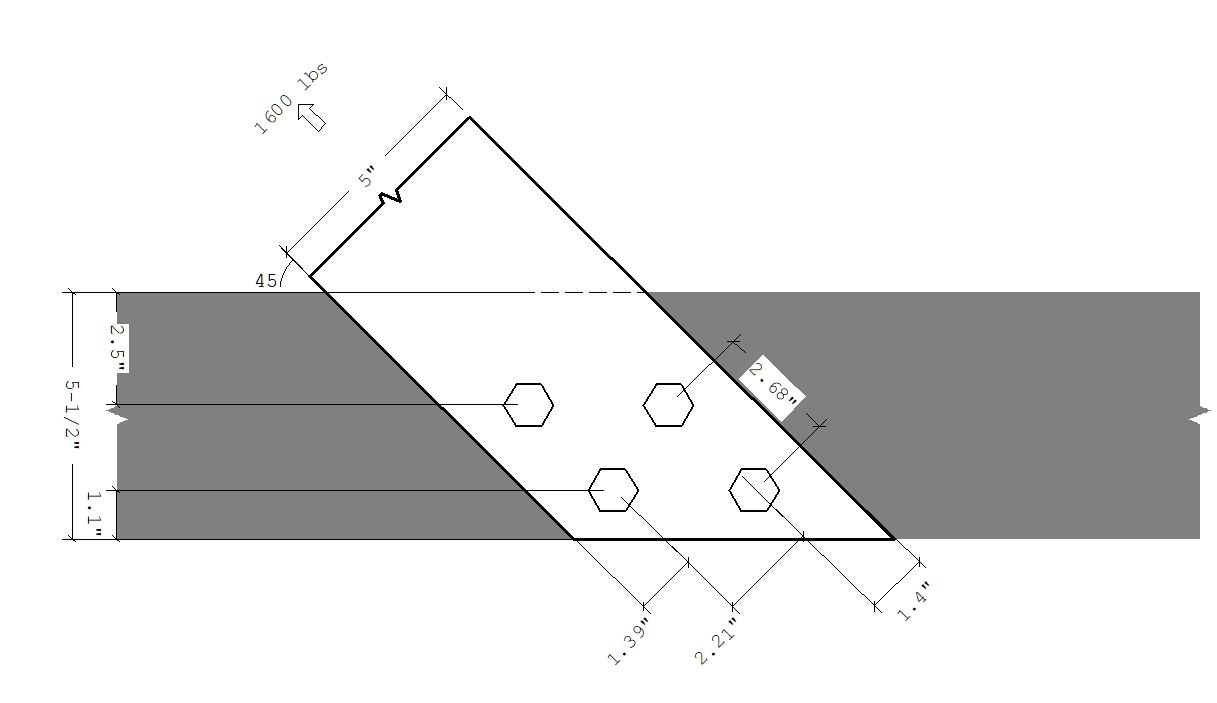
\includegraphics[width=0.650\linewidth]{C:/Users/rodhh/Dropbox/projects/residence_remodel/rivtcalcs0001/docs/d03_models/brace1.jpg}\hfill}

\textbf{Brace plate reinforcement (two-bolt rows shown - one row analyzed)} \hfill {[} Fig: 0302.08 {]}

\begin{quote}
\begin{alltt}
One Steel Side Member Bolted at Angle To Main Member

 Connection Data:
    Main:
       Lumber-soft  D.Fir-L No.1  dry seasoned 5.50 x 5.50"
       Member extends indefinitely, and end assumed to be free.
    Side Plate:
       ASTM A36 Grade A Steel   0.1250 x 5.00"
       End is flush with edge of main member.
    Side member is sloped 135.0 degrees with respect to the main member.

    Temperature (T) : T <= 100 deg F

    Loads:
       Along side member:  1600 lbs   ten minutes duration in tension.

 Connector Design:
    Fasteners:
       Bolt diameter: 5/8"
       2 rows of 2 Bolts =  4 Bolts
       Row Spacing:          2.21"
       Bolt spacing in row:  2.68"

 Design Results using NDS 2015:
    Parallel to Grain:
       Load:                     P  = -1131 lbs
       Row tear out capacity     Rt = 19802 lbs  Ratio: 0.06
    Perpendicular to Grain:
       Lateral load:             Q  =  1131 lbs
    Resultant:
       Combined lateral load:    N  =  1600 lbs at 45.0 degrees
       Lateral capacity:         Z' =  3889 lbs  Ratio: 0.41

 ===============================================================
 Only one bolt per row is used so the lateral capacity is
 reduced by a factor of two.

 =>  DC ratio = .82
 ===============================================================
 Additional Data:
    Adjustment factors:
    CD     CM     Ct     Cg   Cdelta   Cd    Cst    Cft
    1.60   1.00   1.00   0.99   0.76    -      -     1.00

    Yield Limit Values (lbs):
       Im        Is        II        IIIm      IIIs      IV
       2868      1510      1304      1593       812      1128
\end{alltt}
\end{quote}

\vspace{.2in}   \textbf{Seismic D-C Ratios for Beam Connections}   \hfill\textbf{SECTION 03}
\newline   \vspace{.05in}   {\color{black}\hrulefill}

Check beam to beam angle connection drag force load path.

\noindent{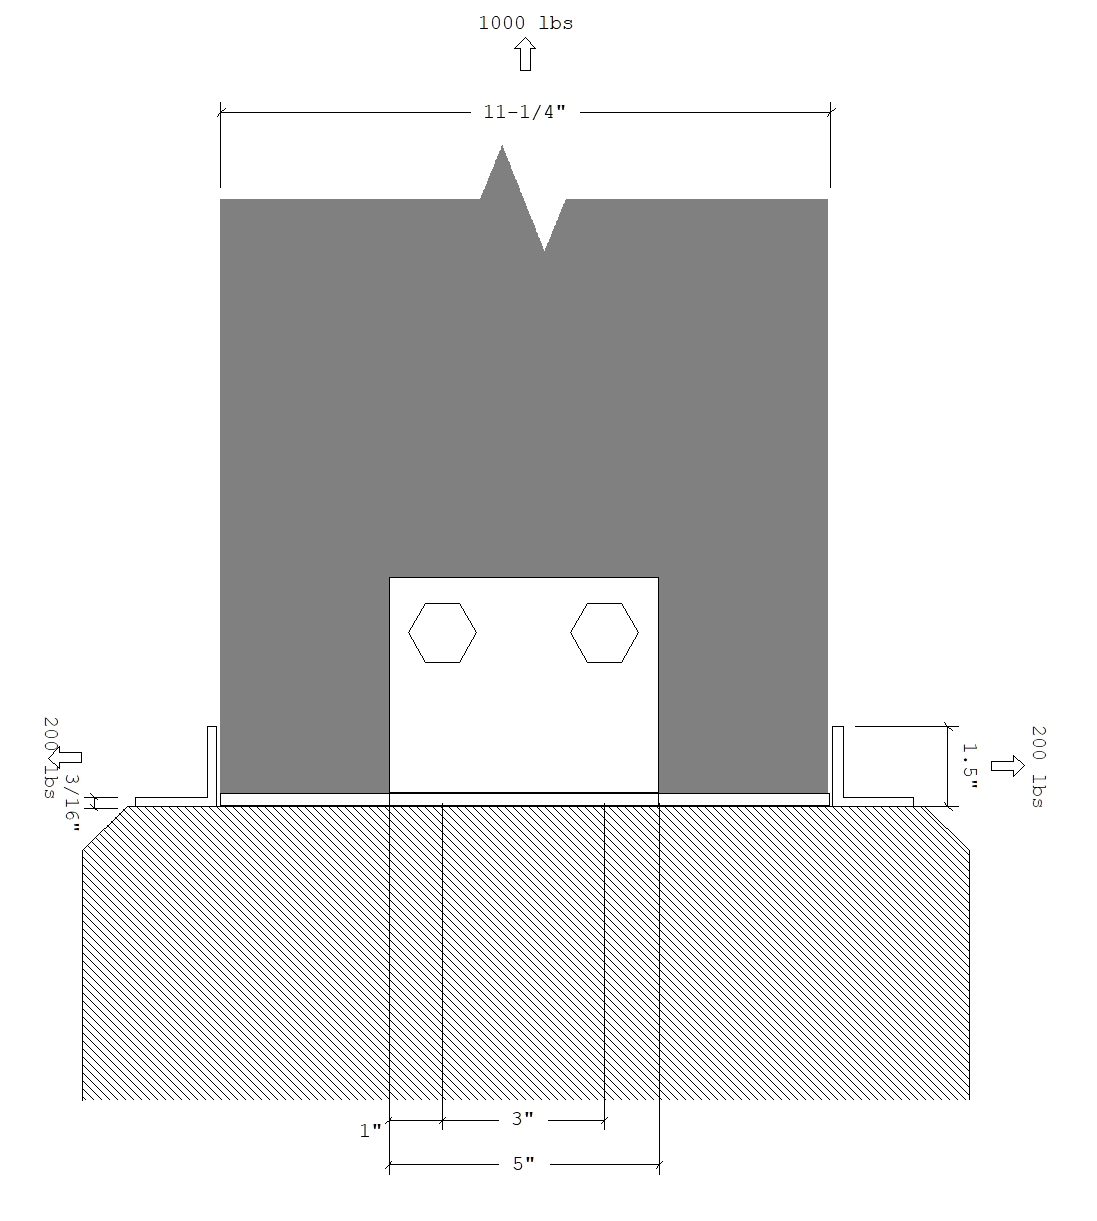
\includegraphics[width=0.500\linewidth]{C:/Users/rodhh/Dropbox/projects/residence_remodel/rivtcalcs0001/docs/d03_models/bmcon.jpg}\hfill}

\begin{quote}
\begin{alltt}
Bolted Column to Base Angle Connector

 Connection Data:
    Column:
       Timber-soft  D.Fir-L No.1  dry seasoned 11.25 x 3.50"

    Temperature (T) : T <= 100 deg F

    Loads:
       Lateral:     200 lbs   ten minutes duration
       Uplift:     1000 lbs   ten minutes duration

 Connector Design:
    Components:                                    Area (sq in)  Weight (lbs)
       2 Side plates:  4.000 x  5.000 x  0.1250"       20.0        0.709
       1 Base plate:   3.500 x 11.250 x  0.2500"       39.4        2.792
       2 Clip Angles: 1-1/2 x 1-1/2 x 3/16 x 0.500 in   1.4        0.077
       Totals:                                         82.3        4.363
       Plate Steel:
          Grade: ASTM A36/A36M       Fy:  35525 psi    Fu:  58000 psi
       Steel Design Checks:
          Each Side Plate:
             Ratio of net area to gross area: 0.675
             Tension in plate: T =   500 lbs   Resistance Tr = 12238 lbs

    Fasteners:
       Face Plate:
          Bolts: ASTM A307     Fy: 45,000 psi     Fu: 60,000 psi
          Bolt diameter: 3/4"
          2 rows of 1 Bolts =  2 Bolts
          Row Spacing:          3"
          Steel Design Checks:
             Shear per bolt:   V =   250 lbs   Resistance:    Vr =  5869 lbs
             Bearing per bolt: B =   250 lbs   Resistance:    Br =  2583 lbs

 Design Results using NDS 2015:
    Load:                     P  =  1000 lbs
    Lateral capacity:         Z' =  5745 lbs  Ratio: 0.17
    Tension capacity net area Tr = 42455 lbs  Ratio: 0.02
    Row tear out capacity     Rt = 18360 lbs  Ratio: 0.05
    Group tear out capacity   Gt = 35758 lbs  Ratio: 0.03
    Horizontal Bearing:
       Lateral load:             Q  =   200 lbs
       Max. bearing load:        Qr =   200 lbs
       Max. bending load:        Yr =   230 lbs

 Additional Data:
    Adjustment factors:
    CD     CM     Ct     Cg   Cdelta   Cd    Cst    Cft
    1.60   1.00   1.00   1.00   0.57    -      -     1.00

    Yield Limit Values (lbs):
       Im        Is        II        IIIm      IIIs      IV
       3675      4078      -          -        3142      4417
\end{alltt}
\end{quote}

Check column connection shear load path to the foundation.

\noindent{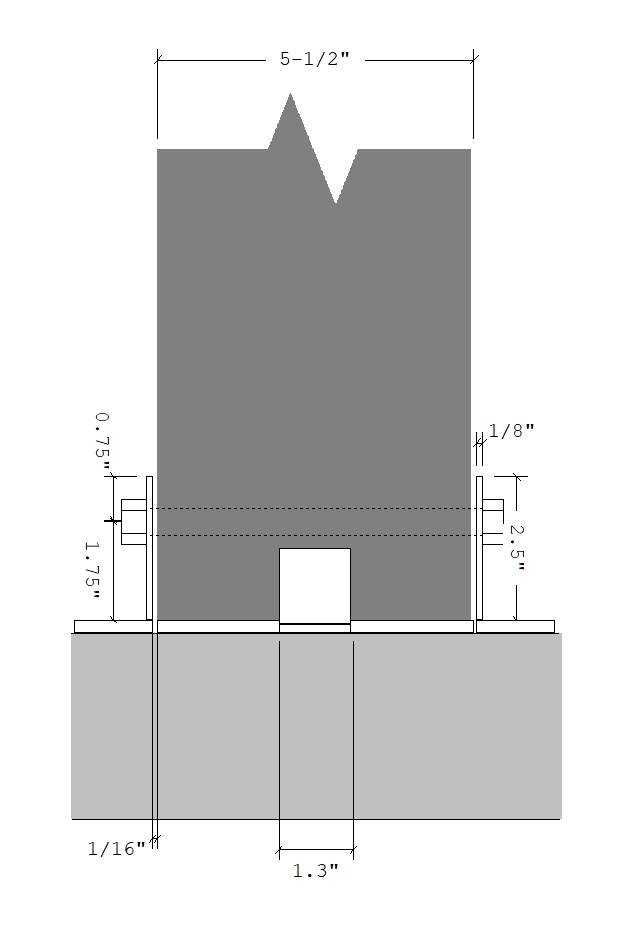
\includegraphics[width=0.500\linewidth]{C:/Users/rodhh/Dropbox/projects/residence_remodel/rivtcalcs0001/docs/d03_models/colcon.jpg}\hfill}

\begin{quote}
\begin{alltt}
Bolted Column to Base Angle Connector

 Connection Data:
    Column:
       Lumber Post  D.Fir-L No.1  dry seasoned 5.50 x 5.50"

    Temperature (T) : T <= 100 deg F

    Loads:
       Lateral:     500 lbs   ten minutes duration
       Uplift:      150 lbs   ten minutes duration

 Connector Design:
    Components:                                    Area (sq in)  Weight (lbs)
       2 Side plates:  2.500 x  1.500 x  0.1250"        3.7        0.133
       1 Base plate:   5.500 x  5.500 x  0.2500"       30.2        2.145
       2 Clip Angles: 1-1/2 x 1-1/2 x 3/16 x 1.281 in   3.6        0.191
       Totals:                                         45.0        2.793
       Plate Steel:
          Grade: ASTM A36/A36M       Fy:  35525 psi    Fu:  58000 psi
       Steel Design Checks:
          Each Side Plate:
             Ratio of net area to gross area: 0.625
             Tension in plate: T =    75 lbs   Resistance Tr =  3399 lbs

    Fasteners:
       Face Plate:
          Bolts: ASTM A307     Fy: 45,000 psi     Fu: 60,000 psi
          Bolt diameter: 1/2"
          1 rows of 1 Bolts =  1 Bolts
          Steel Design Checks:
             Shear per bolt:   V =    75 lbs   Resistance:    Vr =  1590 lbs
             Bearing per bolt: B =    75 lbs   Resistance:    Br =  2040 lbs

 Design Results using NDS 2015:
    Load:                     P  =   150 lbs
    Lateral capacity:         Z' =  1144 lbs  Ratio: 0.13
    Tension capacity net area Tr = 32646 lbs  Ratio: 0.00
    Row tear out capacity     Rt =  2772 lbs  Ratio: 0.05
    Horizontal Bearing:
       Lateral load:             Q  =   500 lbs
       Max. bearing load:        Qr =   500 lbs
       Max. bending load:        Yr =   576 lbs

 Additional Data:
    Adjustment factors:
    CD     CM     Ct     Cg   Cdelta   Cd    Cst    Cft
    1.60   1.00   1.00   1.00   0.50    -      -     1.00

    Yield Limit Values (lbs):
       Im        Is        II        IIIm      IIIs      IV
       3850      2719      -          -        1430      1963
\end{alltt}
\end{quote}

\vspace{.2in}   \textbf{Seismic D-C Ratios for Column Base}   \hfill\textbf{SECTION 04}
\newline   \vspace{.05in}   {\color{black}\hrulefill}

Check shear D-C at column base.

\begin{quote}
\begin{alltt}
==========  ==========  ===========  ================================
variable         value      [value]  description
==========  ==========  ===========  ================================
V_total        1 [kip]    4.45 [KN]  total base shear
V_base      0.25 [kip]  1112.06 [N]  shear distributed over 4 columns
f_c            3 [ksi]  20.68 [MPa]  concrete strength
phi_v             0.85     0.85 [-]  capacity reduction
==========  ==========  ===========  ================================
\end{alltt}
\end{quote}

\textbf{concrete shear strength} \hfill {[} Equ: 0302.01{]}
%
\begin{equation*}
V_{c} = 2 \cdot 3000^{0.5} \cdot \psi \cdot \phi_{v}
\end{equation*}
\begin{quote}
\begin{alltt}
========================  ========  =====
          V_c              phi_v     PSI
========================  ========  =====
0.09 [ksi]  [0.64 [MPa]]  0.85 [-]  [psi]
========================  ========  =====
\end{alltt}
\end{quote}

\textbf{design shear capacity per column} \hfill {[} Equ: 0302.02{]}
%
\begin{equation*}
V_{d} = 4 \cdot 7 \cdot IN \cdot IN \cdot V_{c}
\end{equation*}
\begin{quote}
\begin{alltt}
========================  ===========  ====
          V_d                 V_c       IN
========================  ===========  ====
2.61 [kips]  [0.01 [MN]]  93.11 [psi]  [in]
========================  ===========  ====
\end{alltt}
\end{quote}

\textbf{D-C shear capacity at foundation} \hfill {[} Equ: 0302.03{]}
%
\begin{equation*}
V_{dc} = \frac{V_{base}}{V_{d}}
\end{equation*}
\begin{quote}
\begin{alltt}
====================  =============  ==========
        V_dc               V_d         V_base
====================  =============  ==========
0.10 [-]  [0.10 [-]]  2607.16 [lbs]  0.25 [kip]
====================  =============  ==========
\end{alltt}
\end{quote}

\noindent{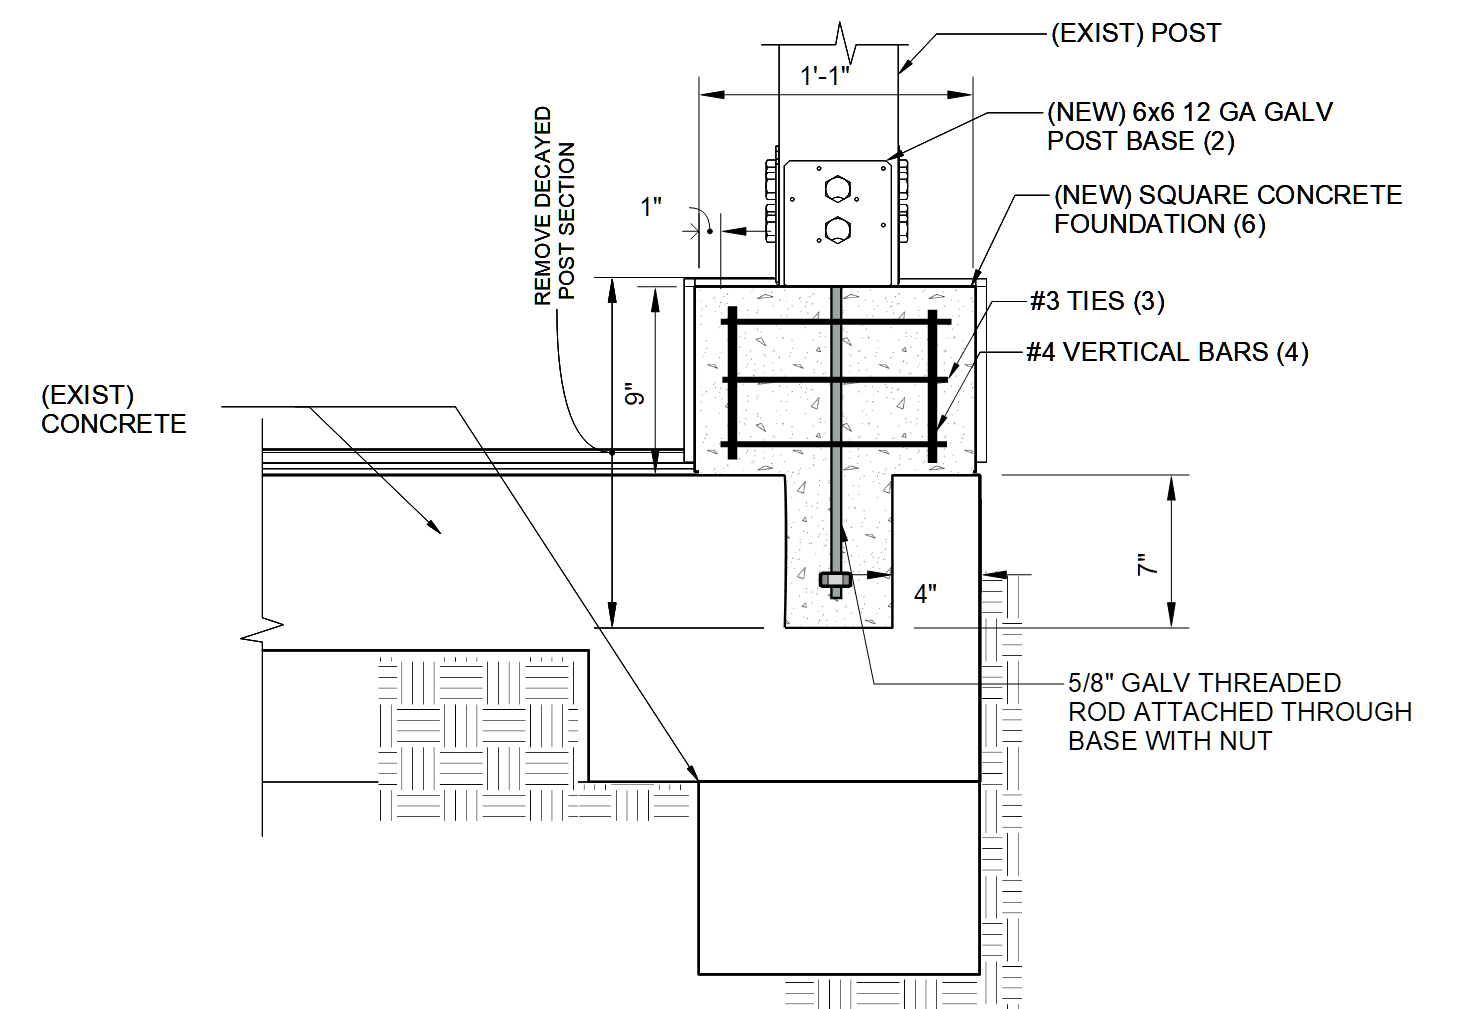
\includegraphics[width=0.700\linewidth]{C:/Users/rodhh/Dropbox/projects/residence_remodel/rivtcalcs0001/docs/d03_models/base_detail.png}\hfill}

Column Base Detail

\end{document}
